%%%%%%%%%%%%%%%%%%%%%%%%%%%%%%%%%%%%%%%%%
% Focus Beamer Presentation
% LaTeX Template
% Version 1.0 (8/8/18)
%
% This template has been downloaded from:
% http://www.LaTeXTemplates.com
%
% Original author:
% Pasquale Africa (https://github.com/elauksap/focus-beamertheme) with modifications by
% Vel (vel@LaTeXTemplates.com)
%
% Template license:
% GNU GPL v3.0 License
%
% Important note:
% The bibliography/references need to be compiled with bibtex.
%
%%%%%%%%%%%%%%%%%%%%%%%%%%%%%%%%%%%%%%%%%

%----------------------------------------------------------------------------------------
%    PACKAGES AND OTHER DOCUMENT CONFIGURATIONS
%----------------------------------------------------------------------------------------

\documentclass{beamer}

\usetheme{focus} % Use the Focus theme supplied with the template
% Add option [numbering=none] to disable the footer progress bar
% Add option [numbering=fullbar] to show the footer progress bar as always full with a slide count

% Uncomment to enable the ice-blue theme
%\definecolor{main}{RGB}{92, 138, 168}
%\definecolor{background}{RGB}{240, 247, 255}

%------------------------------------------------

\usepackage{booktabs} % Required for better table rules
\usepackage{listings}
\usepackage{tikz}
\usetikzlibrary{arrows,automata,positioning,shapes}

\lstset{
    basicstyle=\footnotesize,
    escapeinside=||
}

\newcommand{\todo}[1]{\textcolor{red}{TODO: #1}}

%----------------------------------------------------------------------------------------
%     TITLE SLIDE
%----------------------------------------------------------------------------------------

\title{Introduction to Clang/LLVM}
%\subtitle{Subtitle}
\author{Christian Sharpsten}
\titlegraphic{
\includegraphics[scale=0.6]{images/llvm_logo_derivative.png}}
%\institute{\todo{\\ Institute Name \\ Institute Address}}
\date{01 NOV 2019}

%------------------------------------------------

\begin{document}

%------------------------------------------------

\begin{frame}
    \maketitle
\end{frame}

\begin{frame}{Outline}
    \begin{itemize}
        \item Background
        \begin{itemize}
            \item General Compilation Process
            \item About LLVM
        \end{itemize}
        \vspace{1ex}

        \item LLVM Compilation Process
        \vspace{1ex}

        \item Writing an Optimization Pass
        \begin{itemize}
            \item Building LLVM
            \item A Simple Pass
            \item Taint Tracing to Detect Vulnerable memcpys
            \item Control-Flow Obfuscation
        \end{itemize}
    \end{itemize}
\end{frame}

%----------------------------------------------------------------------------------------
%     SECTION 1
%----------------------------------------------------------------------------------------

\section{Background}

%------------------------------------------------

\begin{frame}{General Compilation Process}
    \begin{overprint}
        \onslide<1>
        \centering
        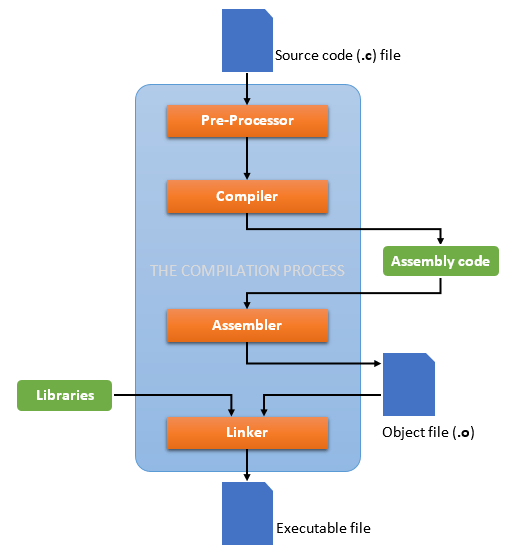
\includegraphics[scale=0.4]{images/high_level_compilation.png}

        \onslide<2>
        \centering
        \begin{tikzpicture}
            \node(a){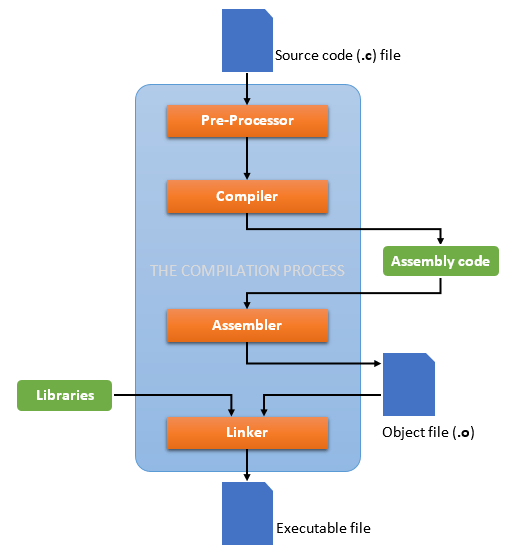
\includegraphics[scale=0.4]{images/high_level_compilation.png}};
            \node at(a.center)[draw, red,line width=2pt,ellipse,minimum width=3cm,minimum height=0.7cm,xshift=-0.2cm,yshift=1.15cm]{};
        \end{tikzpicture}
    \end{overprint}
\end{frame}

\begin{frame}{General Compilation Process}
    \centering
    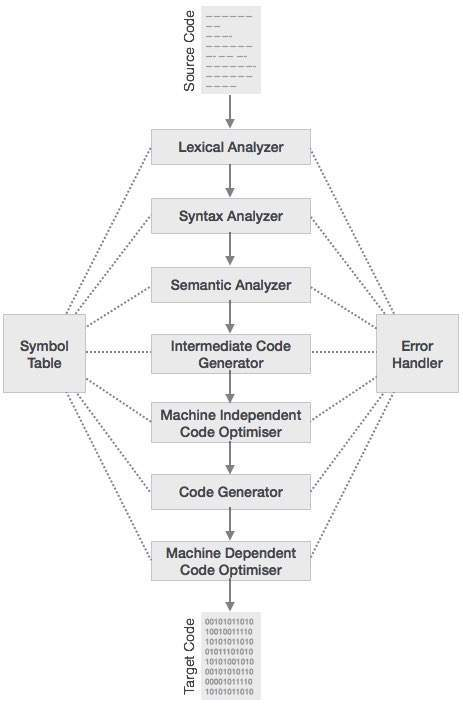
\includegraphics[scale=0.325]{images/low_level_compilation.jpg}
\end{frame}

\begin{frame}[fragile]{General Compilation Process (Lexing)}
    \begin{columns}[T,onlytextwidth]
        \column{0.8\textwidth}
            Convert a stream of characters into a stream of tokens that can be described by a regex.

            \vspace{1ex}
            \begin{lstlisting}[gobble=12]
            int main() {
                return 0;
            }
            \end{lstlisting}

%            \vspace{1ex}
            \begin{lstlisting}[gobble=12]
            TOK_KEYWORD          "int"       1
            TOK_IDENTIFIER       "main"      1
            TOK_L_PAREN          "("         1
            TOK_R_PAREN          ")"         1
            TOK_L_BRACE          "{"         1
            TOK_KEYWORD          "return"    2
            TOK_NUMERIC_CONSTANT "0"         2
            TOK_SEMI             ";"         2
            TOK_R_BRACE          "}"         3
            \end{lstlisting}

        \column{0.2\textwidth}
            \begin{tikzpicture}
                \node(a){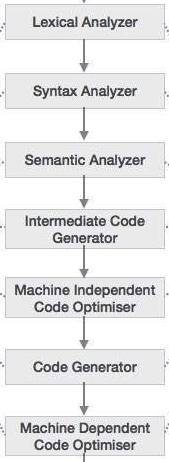
\includegraphics[scale=0.4]{images/low_level_compilation_small.png}};
                \node at(a.center)[draw, red,line width=1pt,ellipse,minimum width=2.5cm,minimum height=0.6cm,yshift=3cm]{};
            \end{tikzpicture}
    \end{columns}
    {\footnotesize \url{llvm-project/clang/include/clang/Basic/TokenKinds.def}}
\end{frame}

\begin{frame}[fragile]{General Compilation Process (Lexing)}
\begin{columns}[T,onlytextwidth]
    \column{0.8\textwidth}
        \begin{overprint}
            \onslide<1>
            Since each token type can be represented as a regex, we can generate a DFA that does the parsing for us. This allows to lex in one pass.

            \todo{picture of DFA}

            \onslide<2>
            In fact, there are tools that do this! Flex is a common tool to do this.

            \begin{lstlisting}[gobble=12,escapeinside=~]
            DIGIT   [0-9]
            ID      [_a-zA-Z][_a-zA-Z0-9]*

            %%
            {DIGIT}+  {
                      printf("Number: %d\n", atoi(yytext));
                      }
            {ID}      {
                      printf("Identifier: %s\n", yytext);
                      }
            int|print {
                      printf("Keyword: %s\n", yytext);
                      }
            %%
            \end{lstlisting}
        \end{overprint}

    \column{0.2\textwidth}
        \begin{tikzpicture}
            \node(a){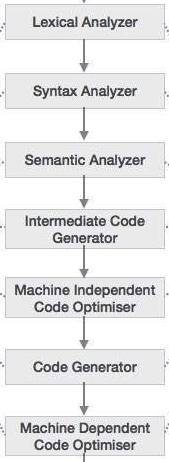
\includegraphics[scale=0.4]{images/low_level_compilation_small.png}};
            \node at(a.center)[draw, red,line width=1pt,ellipse,minimum width=2.5cm,minimum height=0.6cm,yshift=3cm]{};
        \end{tikzpicture}
\end{columns}
\end{frame}

\begin{frame}[fragile]{General Compilation Process (Parsing)}
\begin{columns}[T,onlytextwidth]
    \column{0.8\textwidth}
        \begin{overprint}
            \onslide<1>
            \begin{itemize}
                \item Parsing is the process of building a Parse Tree from the token stream.
                \item The grammar of the language is normally defined by a series of production rules.
            \end{itemize}

            \hspace*{2cm}$EXPR \rightarrow EXPR + TERM$ \\
            \hspace*{2cm}$EXPR \rightarrow EXPR - TERM$ \\
            \hspace*{2cm}$EXPR \rightarrow TERM$ \\
            \hspace*{2cm}$TERM \rightarrow 0$ \\
            \hspace*{2cm}$TERM \rightarrow 1$ \\
            \hspace*{2cm}$TERM \rightarrow ...$ \\
            \hspace*{2cm}$TERM \rightarrow 9$ \\

            If at any point no production is available, we have encountered a parse error.
            \onslide<2>
            Let's build the parse tree for a simple statement.
            \begin{lstlisting}
            a = (5 + 4) - 1
            \end{lstlisting}

            \todo{Parse tree for the above code}

            You can use bison to generate a parser for you!
        \end{overprint}
    \column{0.2\textwidth}
        \begin{tikzpicture}
            \node(a){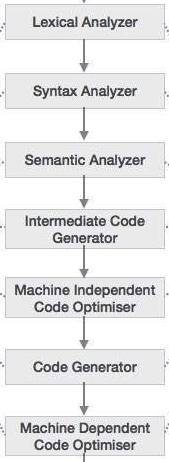
\includegraphics[scale=0.4]{images/low_level_compilation_small.png}};
            \node at(a.center)[draw, red,line width=1pt,ellipse,minimum width=2.5cm,minimum height=0.6cm,yshift=2cm]{};
        \end{tikzpicture}
\end{columns}
\end{frame}

\begin{frame}[fragile]{General Compilation Process (Parsing)}
\begin{columns}[T,onlytextwidth]
    \column{0.8\textwidth}
        \begin{overprint}
            \onslide<1>
            \begin{itemize}
                \item We can then process the parse tree to remove redundant information and perform semantic analysis, like type checking.
                \item This is often where type coercions are introduced.
                \item This phase produces the Abstract Syntax Tree (AST).
            \end{itemize}

            \onslide<2>
            Continuing the earlier example...
            \begin{lstlisting}
            a = (5 + 4) - 1
            \end{lstlisting}

            \todo{Picture of AST for above statement}
        \end{overprint}

    \column{0.2\textwidth}
        \begin{tikzpicture}
            \node(a){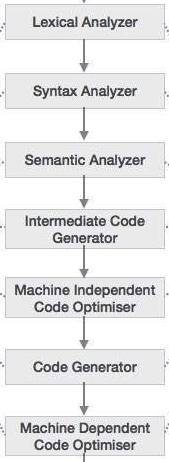
\includegraphics[scale=0.4]{images/low_level_compilation_small.png}};
            \node at(a.center)[draw, red,line width=1pt,ellipse,minimum width=2.5cm,minimum height=0.6cm,yshift=1cm]{};
        \end{tikzpicture}
\end{columns}
\end{frame}

\begin{frame}[fragile]{General Compilation Process (IR Generation)}
\begin{columns}[T,onlytextwidth]
    \column{0.8\textwidth}
        Many compilers generate IR that is in Static Single Assignment (SSA) form - Each variable is assigned exactly once, and every variable is defined before it is used.

        \vspace{1ex}
        \minipage{0.32\textwidth}
            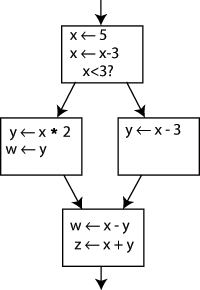
\includegraphics[width=\linewidth]{images/ssa1.png}
        \endminipage\hfill
        \minipage{0.32\textwidth}
            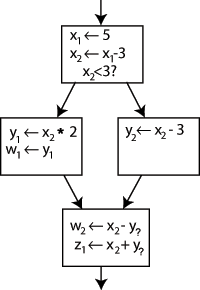
\includegraphics[width=\linewidth]{images/ssa2.png}
        \endminipage\hfill
        \minipage{0.32\textwidth}
            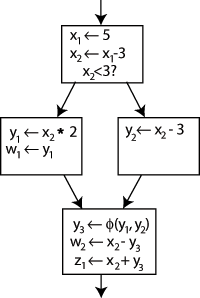
\includegraphics[width=\linewidth]{images/ssa3.png}
        \endminipage\hfill
    \column{0.2\textwidth}
        \begin{tikzpicture}
            \node(a){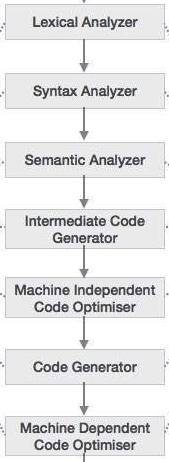
\includegraphics[scale=0.4]{images/low_level_compilation_small.png}};
            \node at(a.center)[draw, red,line width=1pt,ellipse,minimum width=2.5cm,minimum height=0.6cm]{};
        \end{tikzpicture}
\end{columns}
\end{frame}

\begin{frame}[fragile]{General Compilation Process (Optimization)}
\begin{columns}[T,onlytextwidth]
    \column{0.8\textwidth}
        The compiler will run a number of optimization passes. A few of the common ones are listed here.
        \begin{itemize}
            \item Strength Reduction
            \item Constant Propagation
            \item Dead Code Elimination
            \item Loop Invariant Code Motion (Hoisting and Sinking)
            \item Scalar Replacement of Aggregates \& mem2reg
        \end{itemize}
    \column{0.2\textwidth}
        \begin{tikzpicture}
            \node(a){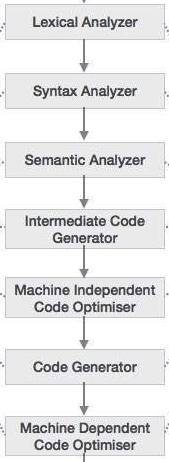
\includegraphics[scale=0.4]{images/low_level_compilation_small.png}};
            \node at(a.center)[draw, red,line width=1pt,ellipse,minimum width=2.5cm,minimum height=0.6cm,yshift=-0.95cm]{};
        \end{tikzpicture}
\end{columns}
\end{frame}

\begin{frame}[fragile]{General Compilation Process (Code Generation)}
\begin{columns}[T,onlytextwidth]
    \column{0.8\textwidth}
        During this phase, the compiler will generate assembly code for the given target.
    \column{0.2\textwidth}
        \begin{tikzpicture}
            \node(a){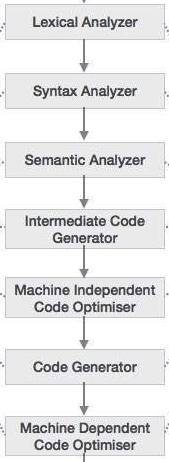
\includegraphics[scale=0.4]{images/low_level_compilation_small.png}};
            \node at(a.center)[draw, red,line width=1pt,ellipse,minimum width=2.5cm,minimum height=0.6cm,yshift=-1.925cm]{};
        \end{tikzpicture}
\end{columns}
\end{frame}

\begin{frame}[fragile]{General Compilation Process (Optimization)}
\begin{columns}[T,onlytextwidth]
    \column{0.8\textwidth}
        Depending on how the backend code generator is implemented, the compiler may apply target-specific optimizations.
    \column{0.2\textwidth}
        \begin{tikzpicture}
            \node(a){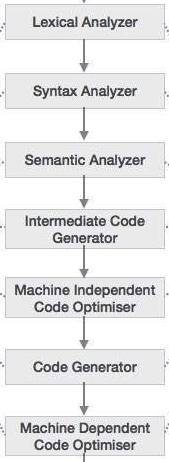
\includegraphics[scale=0.4]{images/low_level_compilation_small.png}};
            \node at(a.center)[draw, red,line width=1pt,ellipse,minimum width=2.5cm,minimum height=0.6cm,yshift=-2.9cm]{};
        \end{tikzpicture}
\end{columns}
\end{frame}

%------------------------------------------------

\begin{frame}{What is LLVM?}
    LLVM is a ``collection of modular and reusable compiler and toolchain technologies.'' \cite{llvm_org}
    \vspace{1em}

    LLVM is composed of multiple sub-projects including:
    {\footnotesize
    \begin{enumerate}
        \item \textbf{LLVM Core} - A set of libraries implementing an optimizer and code generators for common CPUs
        % AArch64, AMDGPU, ARM, BPF, Hexagon, Mips, MSP430, NVPTX, PowerPC, Sparc, SystemZ, X86, XCore
        \item \textbf{Clang} - A front-end compiler
        \item \textbf{LLDB} - A native debugger
        \item \textbf{libc++} - A C++14 compliant STL
        \item \textbf{compiler-rt} - Compiler run-time libraries (intrinsics, ASAN, TSAN, MSAN, etc.)
        % ASAN - Detect OOB accesses, UAF, double free, etc.
        % TSAN - Detect race conditions (experimental)
        % MSAN - Detect uninitialized reads
        \item \textbf{klee} - A symbolic executor
        \item \textbf{LLD} - A drop-in replacement for system linkers such as \texttt{ld}
    \end{enumerate}
    }
\end{frame}

\begin{frame}{Why LLVM?}
    Why is LLVM interesting?
    \begin{itemize}
        \item Modular
        \item Easy to hack on
        \item It has a JIT Engine
        \item Can cross-compile for multiple architectures with one build
    \end{itemize}

    \vspace{1cm}
    LLVM has been used in a number of open source tools:
    \begin{itemize}
        \item Keystone
        \item Capstone
        \item McSema
    \end{itemize}
\end{frame}

\begin{frame}{LLVM Core Tools}
    \textbf{LLVM Core} includes a number of tools:

    \todo{flow chart of tools}

    C Source -> Clang -> LLVM bc -> opt -> LLVM bc -> llc -> .o native code

    LLVM IR -> llvm-as -> LLVM bc

    LLVM bc -> llvm-dis -> LLVM IR
\end{frame}

%----------------------------------------------------------------------------------------
%     SECTION 2
%----------------------------------------------------------------------------------------

\section{LLVM Compilation Process}

%------------------------------------------------

\begin{frame}[fragile]{Clang: Pre-processing, Lexing, and Parsing}
    \begin{lstlisting}[gobble=4]
    int main(void) {
        int a = 5 + 2;
        return a;
    }
    \end{lstlisting}

    \begin{lstlisting}[gobble=4,escapeinside=~]
    $ clang -Xclang -ast-dump test.c
    TranslationUnitDecl <<invalid sloc>> <invalid sloc>
    |-...
    |-...
    `-FunctionDecl <test.c:1:1, line:4:1> line:1:5 main 'int (void)'
      `-CompoundStmt <col:16, line:4:1>
        |-DeclStmt <line:2:5, col:18>
        | `-VarDecl <col:5, col:17> col:9 used a 'int' cinit
        |   `-BinaryOperator <col:13, col:17> 'int' '+'
        |     |-IntegerLiteral <col:13> 'int' 5
        |     `-IntegerLiteral <col:17> 'int' 2
        `-ReturnStmt <line:3:5, col:12>
          `-ImplicitCastExpr <col:12> 'int' <LValueToRValue>
            `-DeclRefExpr <col:12> 'int' lvalue Var 'a' 'int'
    \end{lstlisting}
\end{frame}

\begin{frame}[fragile]{Clang: IR Code Generation}
    Use the \texttt{-emit-llvm} option to enable bitcode generation.

    \begin{lstlisting}[gobble=4]
    $ clang -c -emit-llvm test.c -o test.bc
    $ llvm-dis < test.bc
    ; ModuleID = '<stdin>'
    source_filename = "test.c"
    target datalayout = "e-m:e-i64:64-f80:128-n8:16:32:64-S128"
    target triple = "x86_64-unknown-linux-gnu"

    ; Function Attrs: noinline nounwind optnone uwtable
    define dso_local i32 @main() #0 {
    entry:
    %retval = alloca i32, align 4
    %a = alloca i32, align 4
    store i32 0, i32* %retval, align 4
    store i32 7, i32* %a, align 4
    %0 = load i32, i32* %a, align 4
    ret i32 %0
    }
    ...
    \end{lstlisting}
\end{frame}

\begin{frame}{Clang: IR Code Generation}
    The data layout string describes how data is to be laid out in memory. Elements are separated by the minus sign.

    \vspace{1em}
    \footnotesize
    \texttt{target datalayout = "e-m:e-i64:64-f80:128-n8:16:32:64-S128"}

    \vspace{1ex}
    \begin{tabular}{l | l c}
        \toprule
        Spec        & Description & Value \\
        \toprule
        e           & Endianness & little-endian \\
        m:e         & IR Name Mangling Type & ELF mangling \\
        i64:64      & Alignment for 64-bit integers (bits) & 64 \\
        f80:128     & Alignment for 80-bit floats (bits)    & 128 \\
        n8:16:32:64 & Set of native integer widths for the CPU (bits) & 8, 16, 32, 64 \\
        S128        & Stack Alignment (bits) & 128 \\
        \bottomrule
    \end{tabular}
\end{frame}

%------------------------------------------------

\begin{frame}{opt: Optimization}
How to view passes?
How to run one pass?
Module/Function/BB passes
\end{frame}

%------------------------------------------------

\begin{frame}{llc: Code Generation}
Tablegen
DAG and Legalization
Register allocation
Arch-specific optimizations?
\end{frame}

%----------------------------------------------------------------------------------------
%     SECTION 3
%----------------------------------------------------------------------------------------

\section{Writing an Optimization Pass}

%------------------------------------------------

\begin{frame}{Building LLVM}
    \begin{itemize}
        \item LLVM switched from svn to a single git monorepo as of 21 OCT 2019 (exciting!)
        \item LLVM uses CMake. You can control the build in a number of ways:
        \begin{itemize}
            \item Generator (Ninja, Unix Makefiles, VS, Xcode)
            \item Build type (Debug, Release, RelWithDebInfo, MinSizeRel)
            \item Enabled sub-projects (test suite, libcxx, lldb, lld, etc.)
            \item Backend targets (X86, Mips, PowerPC, etc.)
        \end{itemize}
        \item Depending on which features you enable, LLVM can take a long time to compile.
    \end{itemize}
\end{frame}

%------------------------------------------------

\begin{frame}[fragile]{Building LLVM}
    For this exercise, we only need to build Clang and the X86 backend.

    \begin{lstlisting}[gobble=4]
    $ git clone https://github.com/llvm/llvm-project.git |\pause|
    $ cd llvm-project && git checkout llvmorg-9.0.0 |\pause|
    $ mkdir build && cd build |\pause|
    $ cmake -G Ninja                    \
        -DLLVM_ENABLE_PROJECTS='clang'  \
        -DCMAKE_BUILD_TYPE=Debug        \
        -DLLVM_TARGETS_TO_BUILD=X86
        ../llvm |\pause|
    $ time ninja

    \end{lstlisting}
\end{frame}

%------------------------------------------------

\begin{frame}{Building LLVM}
    LLVM can take a while to compile...

    \begin{table}
        \footnotesize
        \centering
        \begin{tabular}{l c c c | c c}
            \toprule
            Generator & Build Type & Sub-Projects & Targets & Time (m) & Size (GB) \\
            \toprule
            \textbf{Ninja} & \textbf{Debug} & \textbf{Clang} & \textbf{X86} & \textbf{120.15} & \textbf{44.0} \\
            Ninja      & Release & Clang & X86 & 75.03  & 1.7  \\
            Ninja      & Debug   & Clang & All & 205.65 & 59.5 \\
            Ninja      & Release & Clang & All & 106.33 & 2.5  \\
            Make       & Release & Clang & X86 & 433.30 & 1.8  \\
            Make (-j8) & Release & Clang & X86 & 77.13  & 1.7  \\
            \bottomrule
        \end{tabular}
        \caption{\footnotesize LLVM Compile Time Benchmarks (Ubuntu 18.04 VM, 6 cores, 16GB RAM)}
    \end{table}
    % Commands used to benchmark:
    %   cmake -G Ninja -DLLVM_ENABLE_PROJECTS='clang' -DCMAKE_BUILD_TYPE=Debug -DLLVM_PROJECTS_TO_BUILD=X86 ../llvm && time ninja
    %   cmake -G Ninja -DLLVM_ENABLE_PROJECTS='clang' -DCMAKE_BUILD_TYPE=Release -DLLVM_PROJECTS_TO_BUILD=X86 ../llvm && time ninja
    %   cmake -G Ninja -DLLVM_ENABLE_PROJECTS='clang' -DCMAKE_BUILD_TYPE=Debug ../llvm && time ninja
    %   cmake -G Ninja -DLLVM_ENABLE_PROJECTS='clang' -DCMAKE_BUILD_TYPE=Release ../llvm && time ninja
    %   cmake -G 'Unix Makefiles' -DLLVM_ENABLE_PROJECTS='clang' -DCMAKE_BUILD_TYPE=Debug -DLLVM_TARGETS_TO_BUILD=X86 ../llvm && time make
    %   cmake -G 'Unix Makefiles' -DLLVM_ENABLE_PROJECTS='clang' -DCMAKE_BUILD_TYPE=Debug -DLLVM_TARGETS_TO_BUILD=X86 ../llvm && time make -j8

    Keep in mind that debug artifacts can be quite large as well.
\end{frame}

\begin{frame}[fragile]{Building LLVM}
    \begin{alertblock}{High Memory Usage}
        Watch out for out-of-memory errors when linking. Restart ninja/make with less threads if a link process is killed.
    \end{alertblock}

    \vspace{-2ex}

    \begin{overprint}
        \onslide<1>
        \begin{lstlisting}[gobble=8]
        [2361/2742] Linking CXX shared module
            lib/CheckerOptionHandlingAnalyzerPlugin.so
        FAILED: lib/CheckerOptionHandlingAnalyzerPlugin.so
        : && /usr/bin/c++ -fPIC -fPIC ...
        ...
        collect2: fatal error: ld terminated with signal 9 [Killed]
        compilation terminated.
        ninja: build stopped: subcommand failed.
        \end{lstlisting}

        \onslide<2>
        \begin{lstlisting}[gobble=8]
        [2359/2742] Linking CXX executable bin/clang-diff
        FAILED: bin/clang-diff
        : && /usr/bin/c++  -fPIC -fvisibility-inlines-hidden ...
        ...
        /usr/bin/ld: BFD (GNU Binutils for Ubuntu) 2.30 internal error,
            aborting at ../../bfd/merge.c:908 in
            _bfd_merged_section_offset

        /usr/bin/ld: Please report this bug.

        collect2: error: ld returned 1 exit status
        ninja: build stopped: subcommand failed.
        \end{lstlisting}

        \vspace{-2ex}
        \rule{3cm}{0.5pt}

        {\footnotesize \url{https://bugs.debian.org/cgi-bin/bugreport.cgi?bug=874674}}
    \end{overprint}
\end{frame}

%------------------------------------------------

\begin{frame}[fragile]{LLVM IR}
    LLVM comes with IR and tablegen syntax highlighting for vim, emacs, and vscode, among other editors.

    \vspace{1cm}

    \begin{lstlisting}[gobble=4]
    $ cd ~/.vim
    $ ln -s ~/llvm-project/llvm/utils/vim/
            {ftdetect,ftplugin,indent,syntax}
    \end{lstlisting}
\end{frame}

\begin{frame}{LLVM IR}
    use/def
    Everything is a value and a use
    CallInst vs InvokeInst (exception handling)
\end{frame}

\begin{frame}{LLVM IR}
    C code for a short sample
\end{frame}

\begin{frame}{LLVM IR}
    IR for the same sample
\end{frame}

%------------------------------------------------

\begin{frame}{Writing a Pass (Hello World)}
    Module vs Function vs BasicBlock pass
    LoopPass RegionPass and MachineFunctionPass
\end{frame}

\begin{frame}{Writing a Pass (Hello World)}
    Hello world pass
\end{frame}

\begin{frame}{Writing a Pass}
    Builder API
\end{frame}

\begin{frame}{Writing a Pass}
    \todo{Any other interesting things?}
\end{frame}

%------------------------------------------------

\begin{frame}{Writing a Pass (\_\_\_\_)}
    \todo{Bogus arguments? Constant obfuscation? Detect vuln strcpy? Taint tracing?}
\end{frame}

%------------------------------------------------

\begin{frame}{ExtractBB Pass}
    Liveness analysis
\end{frame}

\begin{frame}{ExtractBB Pass}
    Demo with IDA screenshots
\end{frame}

%------------------------------------------------

\begin{frame}{Columns}
    \begin{columns}
        \column{0.5\textwidth}
            This text appears in the left column and wraps neatly with a margin between columns.

        \column{0.5\textwidth}
            \includegraphics[width=\linewidth]{Images/placeholder.jpg}
    \end{columns}
\end{frame}

%------------------------------------------------

\begin{frame}{Lists}
    \begin{columns}[T, onlytextwidth] % T for top align, onlytextwidth to suppress the margin between columns
        \column{0.33\textwidth}
            Items:
            \begin{itemize}
                \item Item 1
                \begin{itemize}
                    \item Subitem 1.1
                    \item Subitem 1.2
                \end{itemize}
                \item Item 2
                \item Item 3
            \end{itemize}

        \column{0.33\textwidth}
            Enumerations:
            \begin{enumerate}
                \item First
                \item Second
                \begin{enumerate}
                    \item Sub-first
                    \item Sub-second
                \end{enumerate}
                \item Third
            \end{enumerate}

        \column{0.33\textwidth}
            Descriptions:
            \begin{description}
                \item[First] Yes.
                \item[Second] No.
            \end{description}
    \end{columns}
\end{frame}

%------------------------------------------------

\begin{frame}[focus]
    Questions?
\end{frame}

%----------------------------------------------------------------------------------------
%     CLOSING/SUPPLEMENTARY SLIDES
%----------------------------------------------------------------------------------------

\appendix

\begin{frame}{References}
    \nocite{*} % Display all references regardless of if they were cited
    \bibliography{references.bib}
    \bibliographystyle{plain}
\end{frame}

%------------------------------------------------

\begin{frame}{Backup Slide}
    This is a backup slide, useful to include additional materials to answer questions from the audience.
    \vfill
    The package \texttt{appendixnumberbeamer} is used to refrain from numbering appendix slides.

    \todo{LTO?}
\end{frame}

%----------------------------------------------------------------------------------------

\end{document}
